\chapter{Порождение признаков с помощью метамоделей}


\section{Problem Statement}
Временные ряды акселерометра образуют множество~$\mathcal{S}$ сегментов~$s$ фиксированной длины~$T$:
\begin{equation}
s = [x_1, \dots, x_T]^{T} \in \bbR^T.
\label{eq::time_series}
\end{equation}
Необходимо построить модель классификации~$f: \bbR^T \rightarrow Y$, которая будет ставить в соответствие каждому сегменту из множества~$\mathcal{S}$ метку класса из конечного множества~$Y$.
Обозначим за
\begin{equation}
	\mathcal{D} = \{(s_i, y_i)\}_{i=1}^m
	\label{eq::sample}
\end{equation}
исходная выборка, где $s_i \in \mathcal{S}$ и $y_i = f(s_i)\in Y$.

Авторы предлагают построить модель~$f$ в в де суперпозиции $f=f(\mathbf{g})$.
Функция $\mathbf{g}: \bbR^T \rightarrow \bbR^n$ является отображением из пространства~$\bbR^{T} $ в признаковое пространство~$G \subset \bbR^n$.
Имея функцию порождения признаков~$\mathbf{g}$, преобразуем исходную выборку~\eqref{eq::sample} в
\[
	\mathcal{D}_G = \{(\mathbf{g}_i, y_i)\}_{i=1}^m,
\]
где $\mathbf{g}_i = \mathbf{g}(s_i) \in G$. 

Модель классификации $f=f(\mathbf{g}, \mathbf{\theta})$ параметризована вектором~$\boldsymbol{\theta}$. 
Оптимальные параметры~$\hat{\mathbf{\theta}}$ определяются оптимизацией функции ошибки классификации
\begin{equation}
\hat{\mathbf{\theta}} = \argmin_{\mathbf{\theta}} L(\mathbf{\theta}, \mathcal{D}_G, \mathbf{\mu}).
\label{eq::optimal_classification_params}
\end{equation}
Вектор~$\mathbf{\mu}$ является внешним параметром для заданной модели классификации. 
Примеры таких параметров и функций ошибки для различных моделей классификации приведены ниже.

Чтобы сравнить качество классификации с прошлыми результатами~\cite{karasikov2016feature,ivkin2015ts}, в качестве метрики качества используется точность классификации:
\begin{equation}
	\mathrm{accuracy} = \frac{1}{m} \sum_{i=1}^{m} \left[f\left(\mathbf{g}(s_i), \hat{\mathbf{\theta}} \right)= y_i\right].
	\label{eq::accuracy}
\end{equation}

\section{Порождение признаков}

Цель данной работы~--- провести сравнение различных подходов к генерации признаков.
В этом разделе проводится анализ рассматриваемых методов.

\subsubsection{Экспертные функции.}
В качестве базового подхода будем использовать экспертные функции как функции порождения признаков.
Экспертные функции~--- это некоторые статистики~$g_j$, где $g_j: \bbR^T \rightarrow \bbR$.
Признаковым описанием~$\mathbf{g}(s)$ объекта~$s$ являются значения заданных экспертных статистик для данного объекта
\[
\mathbf{g}(s) = [g_1(s), \dots, g_n(s)]^{\T}.
\]

В работе~\cite{kwapisz2011activity} авторы предлагают использовать экспертные функции, приведенные в таблице~\ref{tbl::expert_functions}.
Такая процедура порождения признаков генерирует признаковое описание временного ряда~$\mathbf{g}(s) \in \bbR^{40}$.

\begin{table}[ht]
	\centering
	\caption{Expert functions}
	\begin{tabular}{|l|c|}
		\hline
		\textbf{Function description}    & \textbf{Formula} \\ \hline
		Mean                    & $\bar{x} = \frac{1}{T} \sum_{t=1}^{T} x_t$    \\ \hline
		Standard deviation      & $\sqrt{\frac{1}{T} \sum_{t=1}^{T} (x_t - \bar{x})^2}$    \\ \hline
		Mean absolute deviation & $\frac{1}{T} \sum_{t=1}^{T} |x_t - \bar{x}|$    \\ \hline
		Distribution            &  Histogram values with 10 bins    \\ \hline
	\end{tabular}
	\label{tbl::expert_functions}
\end{table}

\subsubsection{Авторегрессионная модель.}
Авторегрессионная модель~\cite{lukashin2003adaptive} порядка $n$
использует параметрическую модель для аппроксимации временного ряда $s$. 
Каждое значение временного ряда приближается линейной комбинацией предыдущих $n-1$ значений
\begin{equation*}
x_t = w_0 + \sum_{j=1}^{n-1} w_j x_{t-j} + \epsilon_t,
\end{equation*}
где $\epsilon_t$~--- регрессионные остатки.
Оптимальные параметры $\hat{\mathbf{w}}$ авторегрессионной модели используются как признаки $\mathbf{g}(s)$.
Данные параметры минимизируют квадратичную ошибку аппроксимации временного ряда и предсказания модели

\begin{equation}
\mathbf{g}(s) = \hat{\mathbf{w}} = \argmin_{\mathbf{w} \in \bbR^{n}} \left( \sum_{t=n}^{T} \|x_t - \hat{x}_t\|^2\right).
\label{eq::autoregressive_description}
\end{equation}
Задача~\eqref{eq::autoregressive_description} эквивалентна задаче линейной регрессии.
Поэтому для каждого временного ряда~$s$ необходимо решить задачу линейной регрессии размера $n$.
Пример аппроксимации временного ряда авторегрессионной моделью представлен на Рис.~\ref{fig::ar_example}.

\begin{figure}[ht]
	\centering
	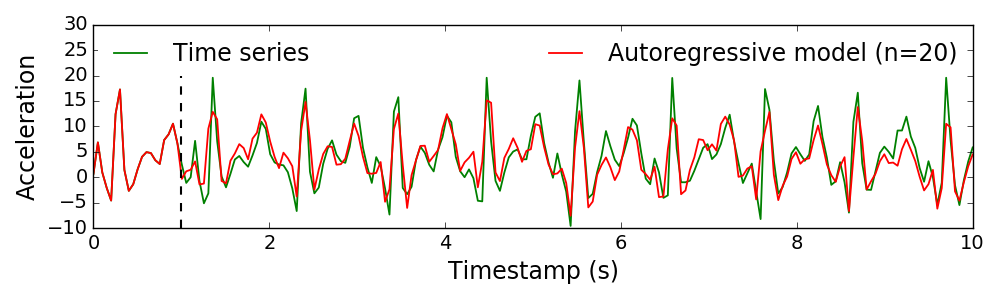
\includegraphics[width=1\linewidth]{figs/ch5/ar_example.png}
	\caption{Time series approximation using autoregressive model with order $n = 20$}
	\label{fig::ar_example}
\end{figure}

\subsubsection{Анализ сингулярного спектра.}
Альтернативной гипотезой порождения признакового пространства для временного ряда является анализ сингулярного спектра (Singular Spectrum Analysis, SSA)~\cite{hassani2007singular}. 
Для каждого временного ряда $s$ из выборки $\mathcal{D}$ строится траекторная матрица:
\[
\mathbf{X} = 
\begin{pmatrix}
x_1 & x_2 & \dots & x_n \\
x_2 & x_3 & \dots & x_{n+1} \\
\dots & \dots & \dots & \dots \\
x_{T-n+1} & x_{T-n+2} & \dots & x_T
\end{pmatrix}.
\]
Здесь ширина окна $n$ является внешним структурным параметром.
Сингулярное разложение матрицы $\mathbf{X}^{\T} \mathbf{X}$:
\[
\mathbf{X}^{\T} \mathbf{X} = \mathbf{U} \mathbf{\Lambda} \mathbf{U}^{\T},
\]
где $\mathbf{U}$~--- унитарная матрица и $\Lambda = \mathrm{diag}(\lambda_1, \dots, \lambda_n)$ причём $\lambda_i$ собственные значения $\mathbf{X}^{\T} \mathbf{X}$. 
Признаковое описание объекта $s$ задаётся спектром матрицы $\mathbf{X}^{\T} \mathbf{X}$:
\[
\mathbf{g}(s) = \left[\lambda_1, \dots, \lambda_n\right]^{\T}.
\]
\subsubsection{Spline Approximation.}
Предлагаемый метод аппроксимирует временные ряды с помощью сплайнов~\cite{deboor1978splines}. Сплайн определяется его параметрами: узлами и коэффициентами.
Предполагается, что узлы сплайна $\{\xi_\ell\}_{\ell=0}^M$ равномерно распределены по временной оси.
Кусочные модели, построенные на отрезках $[\xi_{\ell-1}; \xi_{\ell}]$, заданы коэффициентами $\{\mathbf{w}_\ell\}_{\ell=1}^{M}$.
\begin{figure}[h]
	\centering
	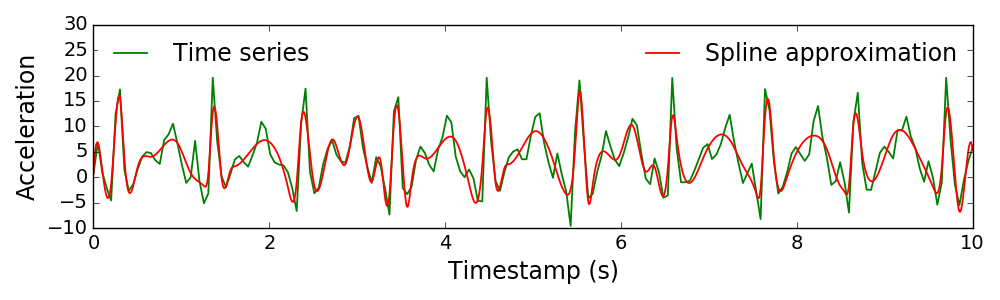
\includegraphics[width=1\linewidth]{figs/ch5/spline_example.png}
	\caption{Time series approximation using three order splines}
	\label{fig::spline_example}
\end{figure}
Оптимальные параметры сплайна являются решением системы с дополнительными условиями равенства производных до второго порядка включительно на концах отрезков.
Обозначим каждый отрезок-сегмент $p_i(t)$ $i = 1, \dots, M$ и весь сплайн $S(t)$. Тогда система уравнений принимает вид
\begin{align*}
S(t) &= \begin{cases}
p_1(t) = w_{10} +w_{11}t + w_{12}t^2 + w_{13}t^3, & t\in [\xi_0, \xi_1],\\
p_2(t) = w_{20} +w_{21}t + w_{22}t^2 + w_{23}t^3, & t\in [\xi_1, \xi_2],\\
\cdots&\cdots \\
p_{M}(t) = w_{L0} +w_{M1}t + w_{M2}t^2 + w_{M3}t^3, & t\in [\xi_{M-1}, \xi_M],					
\end{cases}
\end{align*}
%For $S(t)$ to be an interpolatory cubic spline, we must also have conditions:
\begin{align*}
S(\xi_t) &= x_t, \quad t = 0, \dots, M,\\
p_i'(\xi_i) &= p_{i+1}'(\xi_i),\: p_i''(\xi_i) = p_{i+1}''(\xi_i), \quad i = 1, \dots, M-1,\\
p_i(\xi_{i-1}) &= x_{i-1},\: p_i(\xi_i) = x_i, \quad i = 1, \dots, M.
\end{align*}
Объединение всех параметров сплайна задаёт признаковое описание временного ряда:
\[
\mathbf{g}(s) = \left[\mathbf{w}_1, \dots, \mathbf{w}_{M}\right]^{\T}.
\]

Рис.~\ref{fig::spline_example} показывает аппроксимацию временного ряда с использованием модели сплайнов.
По сравнению с авторегрессионной моделью сплайны строят более гладкую аппроксимацию, используя такое же количество параметров.

\section{Классификация временных рядов}
Для классификации временных рядов будем использовать подход один против всех. 
Для каждого класса обучается бинарный классификатор, и на стадии предсказания объект классифицируется согласно наиболее уверенному классификатору.
Использовались три модели классификации: логистическая регрессия, SVM и случайный лес.

\subsubsection{Логистическая регрессия.}
Оптимальные параметры модели $\hat{\mathbf{w}}, \hat{b}$  в случае логистической регрессии определяются минимизацией функции ошибки~\eqref{eq::optimal_classification_params}

\begin{equation*}
L(\mathbf{\theta}, \mathcal{D}_G, \mu) = \sum_{i=1}^{m} \log\bigl(1 + \exp(-y_i [\mathbf{w}^{\T} \mathbf{g}_i + b])\bigl) + \frac{\mu}{2} \|\mathbf{w}\|^2, \:\:\mbox{where}\:\: \mathbf{\theta}  = \begin{bmatrix}
\mathbf{w} \\ b
\end{bmatrix}.
\end{equation*}

Решающее правило $f(\mathbf{g}, \mathbf{\theta})$~--- знак линейной комбинации описания объекта $\mathbf{g}$ и параметров $\hat{\mathbf{\theta}}$
\begin{equation*}
\hat{y} = f(\mathbf{g}, \hat{\mathbf{\theta}}) = \sgn(\mathbf{g}^{\T} \hat{\mathbf{w}} + \hat{b}).
\end{equation*}

\subsubsection{SVM.}
Оптимизационная задача метода SVM имеет вид
\begin{align*}
\hat{\mathbf{\theta}}  = \begin{pmatrix}
\hat{\mathbf{w}} \\ \hat{b} \\ \hat{\mathbf{\xi}}
\end{pmatrix}= \argmin_{\mathbf{w}, b, \mathbf{\xi}}  \frac{1}{2} \|\mathbf{w}\|^2 + \mu \sum_{i=1}^{m} \xi_i,\:\:
\mbox{s.t.} \:\: &y_i \left(\mathbf{w}^{\T} \mathbf{g}_i + b\right) \geq 1 - \xi_i,\\
&\xi_i \geq 0, \quad 1 \leq i \leq m.
\end{align*}
Целевая функция соответствует функции ошибки классификации $L(\mathbf{\theta}, \mathcal{D}_G, \mu)$.
Предсказание для нового объекта вычисляется аналогично $
\hat{y} = \sgn (\mathbf{g}^{\T} \hat{\mathbf{w}} + \hat{b})$.

\subsubsection{Случайный лес.}
Случайный лес использует идею бэггинга. 
Идея состоит в построении многих слабых, неустойчивых классификатов на подвыборках с возвращениями и усреднения их предсказаний.
Метод предполагает использование в качестве базовых классификаторов моделей с низким смещением и высокой дисперсией. 
Усреднение позволяет уменьшить дисперсию.
В случае случайного леса базовой моделью выступают решающие деревья. Идея бэггинга используется не только для самих объектов, но и для множества признаков.
В данном случае предсказание для нового объекта получается усреднением всех предсказаний отдельных деревьев:

\begin{equation*}
\hat{y} = \sgn \left(\frac{1}{B} \sum_{i=1}^{B} \text{pred}(\mathbf{g}_i) \right),
\end{equation*}
где $B$~--- количество деревьев в композиции.


\section{Эксперимент}
В данной работе эксперименты проводились на двух датасетах временных рядов акселерометра мобильного телефона: WISDM~\cite{wisdm} и USC-HAD~\cite{usc}. 
Акселерометр мобильного телефона проводит измерение ускорения по трём осям с частотой 100 Hz.
Данные WISDM содержат 4321 временной ряд.
Каждый временной ряд прнадлежит к одному из 6 классов. 
Данные USC-HAD содержат 13620 временных рядов, принадлежащих одному из 12 классов.  
В таблице~\ref{tbl::activities_distributions} представлено распределение временных рядов по классам для каждого датасета.
Длина временного ряда равна 200.
На рис.~\ref{fig::ts_example} представлен пример одного из временных рядов.

\begin{table}[!ht]
	\centering
	\caption{Distributions of the classes}
	\subfloat[WISDM]{
		\begin{tabular}{r|l|rr}
			\hline
			&\textbf{Activity}   & \multicolumn{2}{l}{\textbf{\# objects}} \\
			\hline
			1&Standing            &229      &5.30  \% \\
			2&Walking             &1917     &44.36 \% \\
			3&Upstairs            &466      &10.78 \% \\
			4&Sitting             &277      &6.41  \% \\
			5&Jogging             &1075     &24.88 \% \\
			6&Downstairs          &357      &8.26  \% \\
			\hline
			&Total & \multicolumn{2}{l}{4321}  \\
			\hline
	\end{tabular}}
	\hspace{0.5cm}
	\subfloat[USC-HAD]{
		\begin{tabular}{r|l|rr}
			\hline
			&\textbf{Activity} & \multicolumn{2}{l}{\textbf{\# objects}} \\ \hline
			1&Standing            &1167     &8.57  \% \\
			2&Elevator-up         &764      &5.61  \% \\
			3&Walking-forward     &1874     &13.76 \% \\
			4&Sitting             &1294     &9.50  \% \\
			5&Walking-downstairs  &951      &6.98  \% \\
			6&Sleeping            &1860     &13.66 \% \\
			7&Elevator-down       &763      &5.60  \% \\
			8&Walking-upstairs    &1018     &7.47  \% \\
			9&Jumping             &495      &3.63  \% \\
			10&Walking-right       &1305     &9.58  \% \\
			11&Walking-left        &1280     &9.40  \% \\
			12&Running             &849      &6.23  \% \\
			\hline 
			&Total              & \multicolumn{2}{l}{13620}\\ 
			\hline
	\end{tabular}}
	\label{tbl::activities_distributions}
\end{table}

\begin{figure}[!ht]
	\centering
	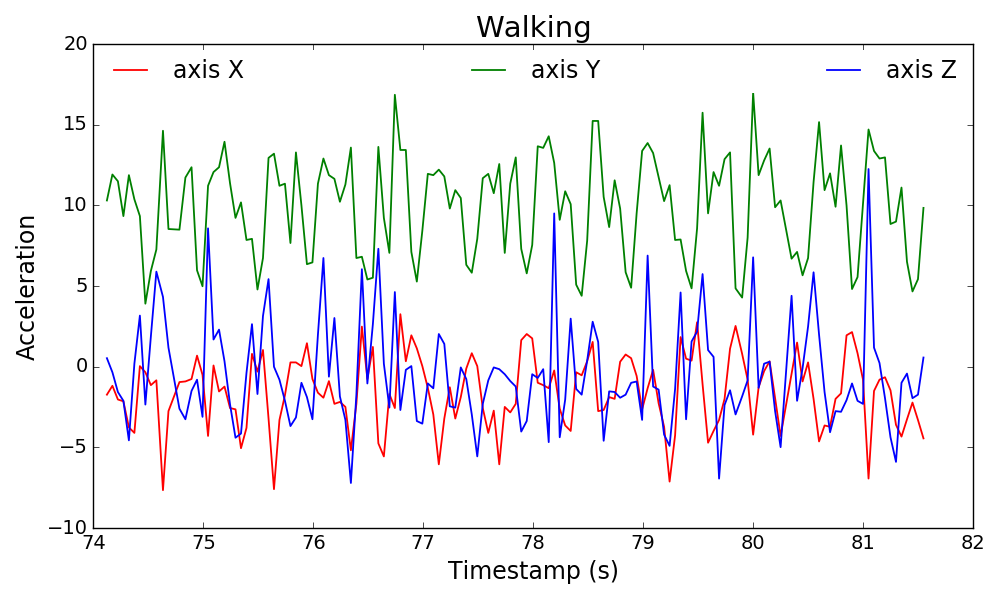
\includegraphics[width=1\linewidth]{figs/ch5/ts_example.png}
	\caption{Time series example}
	\label{fig::ts_example}
\end{figure}

\begin{figure}[!ht]
	\centering
	\subfloat{
		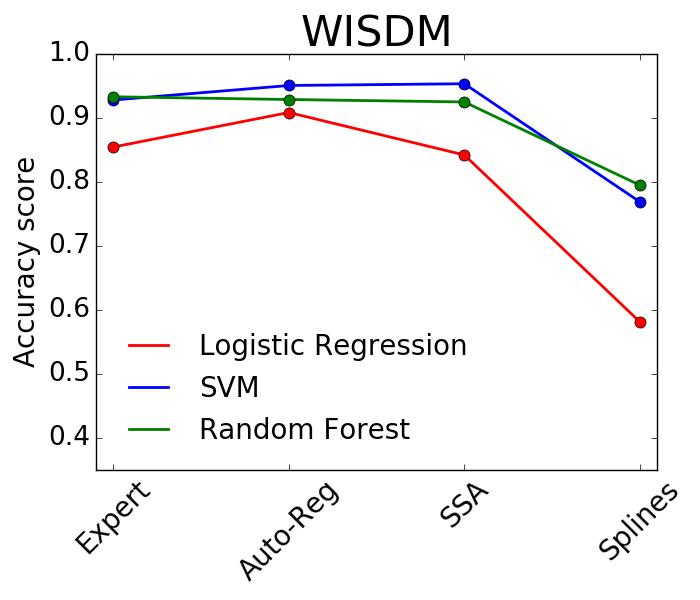
\includegraphics[width=0.49\linewidth]{figs/ch5/wisdm_methods.png}}
	\subfloat{
		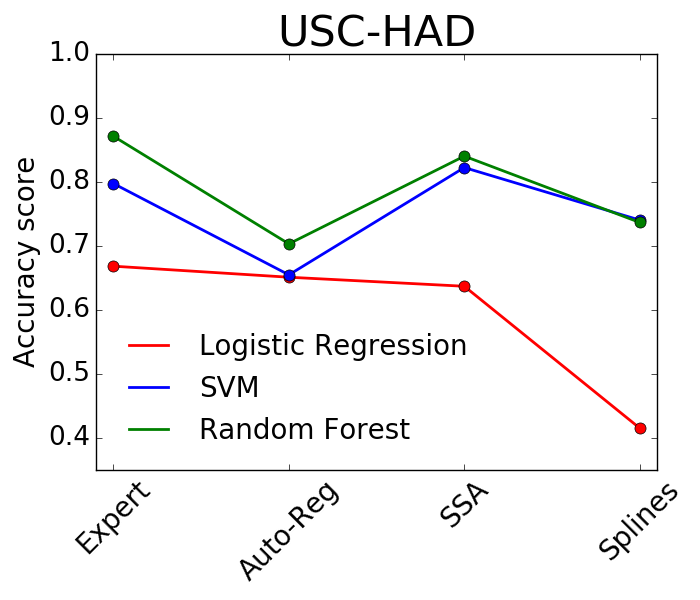
\includegraphics[width=0.49\linewidth]{figs/ch5/uschad_methods.png}}
	\caption{Multiclass accuracy score}
	\label{fig::accuracy_results}
\end{figure}

В эксперименте для каждого датасета были порождены признаки одним из методов: экспертные функции, авторегрессионная модель, SSA и сплайны.
Для каждой процедуры порождения признаквого описания настроивались три модели классификации: логистическая регрессия, SVM и случайный лес.
Внешние структурные параметры (длина авторегрессионной модели $n$, ширина окна SSA $n$, число узлов сплайна $M$) настраивались процедурой кросс-валидации:
\begin{align}\label{cv}
CV(K) = \frac{1}{K}\sum_{k=1}^{K} L(f_k, \mathcal{D}\setminus \mathcal{C}_k),
\end{align}
где $C_k$~---$\frac{K-1}{K}$ доля от всей выборки, используемая для обучения модели $f_k$.
Гиперпараметры $\boldsymbol{\mu}$ моделей классификации были настроаны той же процедурой кросс-валидации.

Первый подход к порождению признаков временных рядов~---экспертные функции.
Основной недостаток такого подхода необходимость экспертного задания функций	 и возможности вычисления их для конкретного датасета.

Авторегрессионная модель требует задания параметра длины модели $n$. 
Процедура кросс-валидации дала наибольшее качество при $n=20$ для обоих датасетов.

Модель SSA была настроена аналошгичной процедурой выбора оптимальных гиперпараметров. Конечная модель имела ширину окна $n=20$.

\begin{figure}[!ht]
	\centering
	\subfloat[WISDM dataset]{
		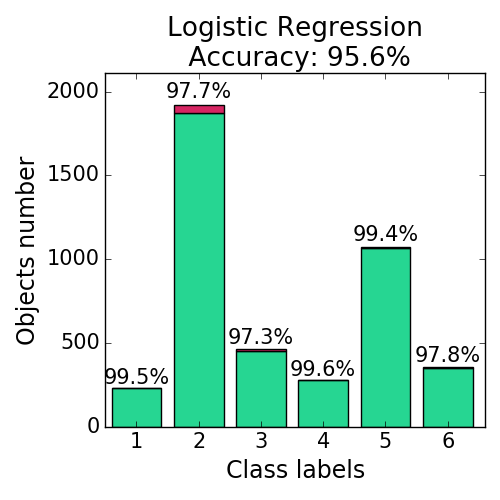
\includegraphics[width=0.33\linewidth]{figs/ch5/hist_wisdm_lr_all.png}}
	\subfloat[USC-HAD dataset]{
		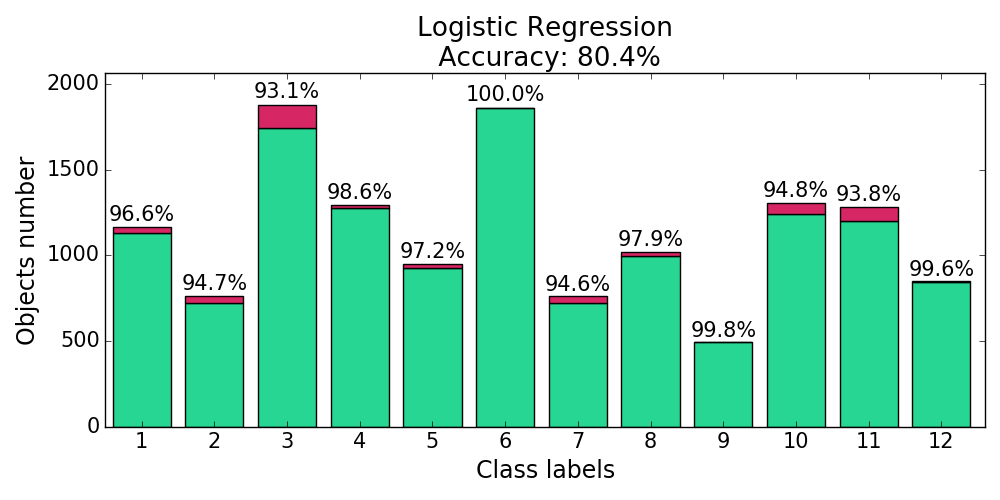
\includegraphics[width=0.66\linewidth]{figs/ch5/hist_uschad_lr_all.png}}\\
	\subfloat[WISDM dataset]{
		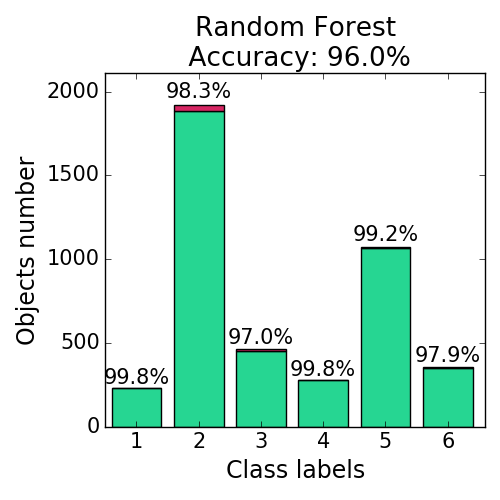
\includegraphics[width=0.33\linewidth]{figs/ch5/hist_wisdm_rf_all.png}}
	\subfloat[USC-HAD dataset]{
		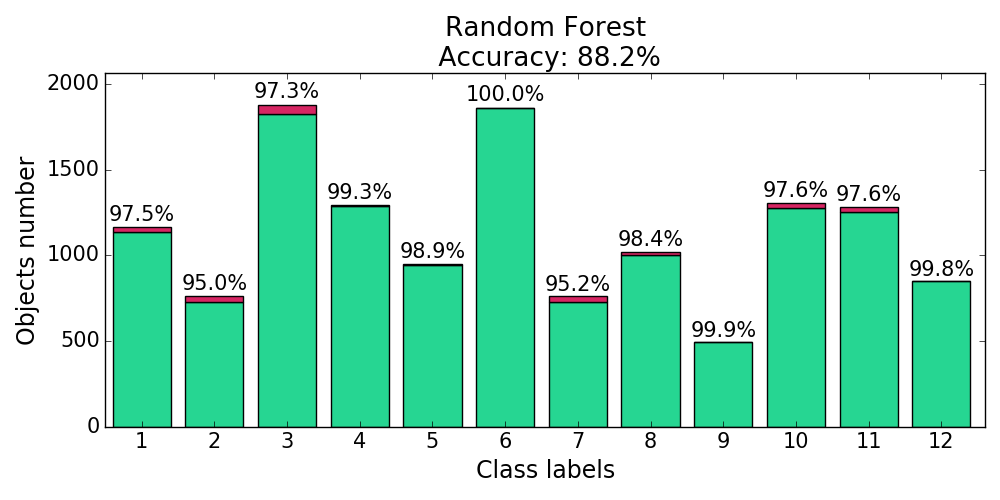
\includegraphics[width=0.66\linewidth]{figs/ch5/hist_uschad_rf_all.png}}\\
	\subfloat[WISDM dataset]{
		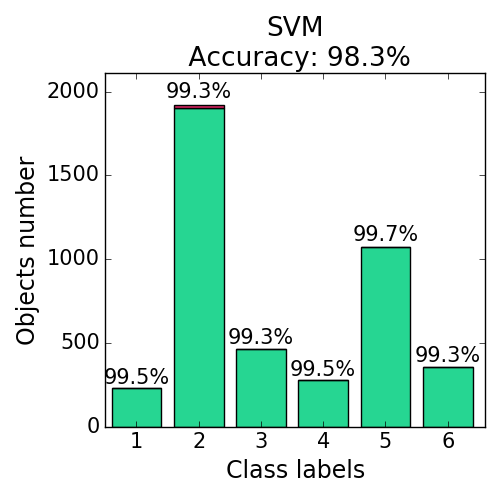
\includegraphics[width=0.33\linewidth]{figs/ch5/hist_wisdm_svm_all.png}}
	\subfloat[USC-HAD dataset]{
		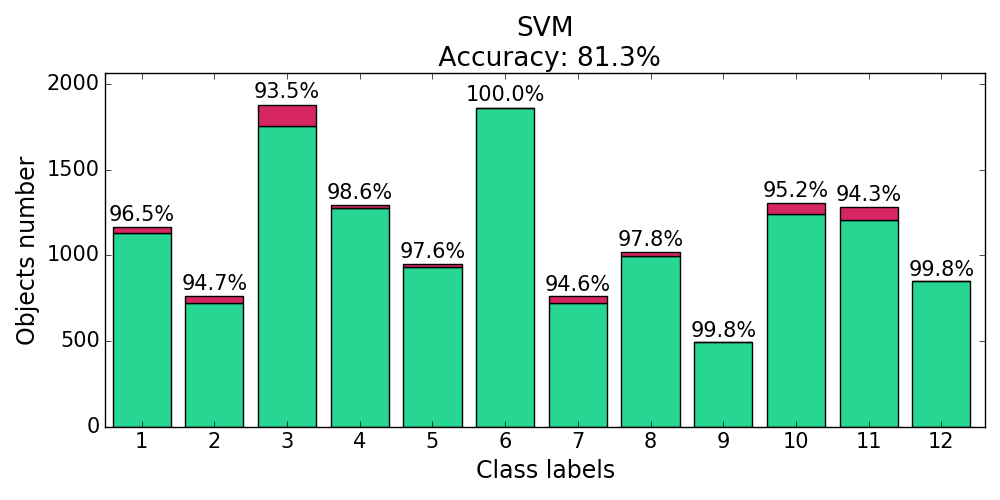
\includegraphics[width=0.66\linewidth]{figs/ch5/hist_uschad_svm_all.png}}\\
	\caption{Accuracy scores of classification of each class using all features}
	\label{fig::feature_union_results}
\end{figure}

Для аппроксимации временных рядов кубическими сплайнами~\cite{deboor1978splines} использовалась библиотека $scipy$. 
Узлы сплайнов $\{\xi_{\ell}\}_{\ell = 1}^M$ были распределены равномерно по временной оси.
Значение параметра $M$ было подобрано на кросс-валидации.

Для обоих датасетов процедуры порождения признаковых описаний дали следующие количества признаков: экспертные функции~---40; авторегрессионная модель~---60; анализ сингулярного спектра~---60; сплайны~---33.

\begin{table}[!ht]
	\centering
	\caption{Binary accuracy scores for WISDM using different feature generation methods: EX~--- Expert, AR~--- Auto-Reg, SSA and  SPL for Splines}
	\footnotesize
	\begin{tabular}{r|rrrr|rrrr|rrrr|}
		& \multicolumn{4}{c|}{\textbf{Logistic Regression}} & \multicolumn{4}{c|}{\textbf{Random Forest}} & \multicolumn{4}{c|}{\textbf{SVM}}          \\ \cline{2-13} 
		& EX   & AR   & SSA   & SPL  & EX  & AR & SSA & SPL & EX & AR & SSA & SPL \\ \hline
		All& 0.85 & 0.91 & 0.84 & 0.58 & 0.93 & 0.93 & 0.92 & 0.79 & 0.93 & 0.95 & 0.95 & 0.77 \\
		Standing& 0.99 & 0.98 & 1.00 & 0.95 & 1.00 & 0.99 & 1.00 & 0.99 & 0.99 & 0.98 & 1.00 & 0.96 \\
		Walking& 0.91 & 0.96 & 0.86 & 0.61 & 0.96 & 0.97 & 0.95 & 0.86 & 0.96 & 0.98 & 0.98 & 0.84 \\
		Upstairs& 0.91 & 0.95 & 0.91 & 0.89 & 0.96 & 0.96 & 0.96 & 0.90 & 0.96 & 0.98 & 0.97 & 0.89 \\
		Sitting& 0.99 & 0.98 & 1.00 & 0.99 & 1.00 & 0.99 & 1.00 & 1.00 & 0.99 & 0.98 & 1.00 & 1.00 \\
		Jogging& 0.98 & 0.99 & 0.99 & 0.80 & 0.99 & 0.99 & 0.99 & 0.92 & 0.99 & 0.99 & 0.99 & 0.93 \\
		Downstairs& 0.93 & 0.96 & 0.94 & 0.92 & 0.96 & 0.97 & 0.96 & 0.92 & 0.96 & 0.98 & 0.97 & 0.92 \\ \hline
	\end{tabular}
	\label{tbl::wisdm_methods_results}
\end{table}

\begin{table}[!ht]
	\centering
	\footnotesize
	\caption{Binary accuracy scores for USC-HAD using different feature generation methods: EX~--- Expert, AR~--- Auto-Reg, SSA and  SPL for Splines}
	\label{my-label}
	\begin{tabular}{r|rrrr|rrrr|rrrr|}
		& \multicolumn{4}{c|}{\textbf{Logistic Regression}} & \multicolumn{4}{c|}{\textbf{Random Forest}} & \multicolumn{4}{c|}{\textbf{SVM}}          \\ \cline{2-13} 
		& EX   & AR   & SSA   & SPL  & EX  & AR & SSA & SPL & EX & AR & SSA & SPL \\ \hline
		All& 0.67 & 0.65 & 0.64 & 0.41 & 0.87 & 0.70 & 0.84 & 0.74 & 0.80 & 0.65 & 0.82 & 0.74 \\
		Standing& 0.94 & 0.94 & 0.92 & 0.89 & 0.98 & 0.94 & 0.97 & 0.98 & 0.95 & 0.94 & 0.97 & 0.96 \\
		Elevator-up& 0.94 & 0.94 & 0.93 & 0.92 & 0.95 & 0.95 & 0.95 & 0.95 & 0.93 & 0.94 & 0.94 & 0.93 \\
		Walking-forward& 0.87 & 0.87 & 0.89 & 0.70 & 0.97 & 0.89 & 0.96 & 0.88 & 0.95 & 0.87 & 0.97 & 0.91 \\
		Sitting& 0.98 & 0.95 & 0.94 & 0.96 & 0.99 & 0.96 & 0.98 & 0.99 & 0.98 & 0.96 & 0.99 & 0.99 \\
		Walking-downstairs& 0.95 & 0.93 & 0.93 & 0.90 & 0.99 & 0.96 & 0.98 & 0.95 & 0.98 & 0.93 & 0.98 & 0.96 \\
		Sleeping& 1.00 & 0.98 & 0.99 & 1.00 & 1.00 & 0.98 & 1.00 & 1.00 & 1.00 & 0.98 & 1.00 & 1.00 \\
		Elevator-down& 0.94 & 0.94 & 0.94 & 0.91 & 0.95 & 0.95 & 0.95 & 0.95 & 0.93 & 0.94 & 0.94 & 0.93 \\
		Walking-upstairs& 0.94 & 0.95 & 0.93 & 0.92 & 0.98 & 0.95 & 0.98 & 0.96 & 0.98 & 0.95 & 0.98 & 0.96 \\
		Jumping& 0.99 & 0.99 & 1.00 & 0.97 & 1.00 & 0.99 & 1.00 & 0.99 & 1.00 & 0.99 & 0.97 & 0.99 \\
		Walking-right& 0.91 & 0.90 & 0.91 & 0.86 & 0.97 & 0.92 & 0.96 & 0.92 & 0.96 & 0.90 & 0.97 & 0.93 \\
		Walking-left& 0.89 & 0.91 & 0.90 & 0.88 & 0.97 & 0.93 & 0.97 & 0.93 & 0.95 & 0.91 & 0.97 & 0.93 \\
		Running& 0.99 & 0.99 & 0.99 & 0.92 & 1.00 & 0.99 & 1.00 & 0.97 & 1.00 & 1.00 & 0.95 & 0.98\\ \hline
	\end{tabular}
	\label{tbl::uschad_methods_results}
\end{table}

На рис.~\ref{fig::accuracy_results} показано качество классификации~\eqref{eq::accuracy} для двух датасетов.
Для данных WISDM сплайны дали самое слабое качество классификации.
Результаты для экспертных функций, авторегрессионной модели и SSA схожи.
Для данных USC-HAD результат более восприимчив к выбору модели классификации. 
Для обоих датасетов логистическая регрессия продемонстрировала наименьшее качество, SVM и случайный лес показали почти одинаковое качество.
Для датасета USC-HAD модель с использованием аппроксимации сплайнами
показала сравнимое с другими методами качество. 

В Табл.~\ref{tbl::wisdm_methods_results} и Табл.~\ref{tbl::uschad_methods_results} представлены результаты классификации~\eqref{eq::accuracy} для каждого класса в отдельности.
Первая строка в обеих таблицах демонстрирует точность по всем классам для каждой модели и процедуры генерации признаков.
Следующие строки соответствуют бинарным точностям по каждому из классов.
Для данных WISDM лучшее качество имеют наименее активные классы, такие как Standing и Sitting. 
Для USC-HAD заметного выделения качества для определенных классов не наблюдается.

Также был проведён эксперимент с использованием объединённого множества всех 193 сгенерированных признаков.
Результаты представлены на Рис.~\ref{fig::feature_union_results}. Соответствие между номера классов и видами активности приведено в Табл.~\ref{tbl::activities_distributions}. 
Объединение признаков для обучения одной модели позволило увеличить качество. 
Для данных WISDM все точности классификации по классам больше $97 \%$, а для USC-HAD выше $93 \%$.
